\subsection{Theoretischer Hintergrund: P Cygni Profil} \label{sec:T-H-P-Cygni}
Betrachtet man bestimmte Emissionslinien eines Sterns, so lässt sich bei einem Stern mit vorhandenem Sternwind ein P Cygni Profil, Abb.\ (\ref{fig:p_cygni_profil}), erkennen.
\begin{figure}[t]
  \centering
  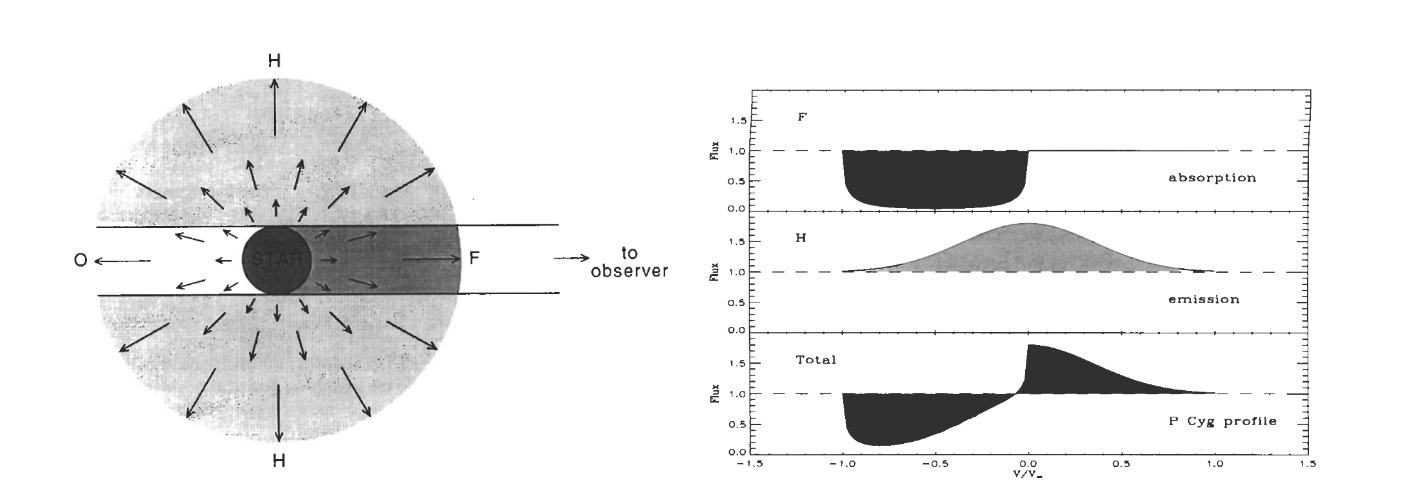
\includegraphics[width=.5\textwidth]{464_p_cygni_profil.png}
  \caption{Das P Cygni Profil eines Sterns. Abzisse: $v/v_\infty$.\cite{anleitung464}} \label{fig:p_cygni_profil}
\end{figure}

Innerhalb des Windes emittiert der Stern Licht.
Dieses Licht wird von dem Sternwind, welcher genau in der Linie zwischen Beobachter und Stern liegt, absorbiert.
Dadurch lässt sich hier eine Verringerung des Flusses feststellen.
Dies erkennt man in Abb.\ (\ref{fig:p_cygni_profil}) in F.
Da sich der Sternwind jenseits des Sterns ausbreitet, wird dort ein größerer Fluss festgestellt, der durch die Emission des Windes selbest hervorgerufen wird.
Dies erkennt man in H.
Hinter dem Stern (relativ zum Beobachter) wird keine Strahlung gemessen, da diese nicht durch den Kern des Sterns zur Seite des Beobachters dringt.
Fügt man F und H zusammen, so ergibt sich eine charakteristische Kurve, die bei Sternen mit Sternwinden auftritt.

Die Absorption ist keine Absorptionslinie, sondern ein Absorptionstrog, da der Sternwind verschiedene Geschwindigkeiten aufweist.
Dabei hat er eine Geschwindigkeit von $-v_\infty$ am äußersten Rand\footnote{Die Bewegung ist relativ zum Beobachter, daher ist die Geschwindigkeit negativ. Die Richtung vom Beobachter weg ist Positiv.} und eine Geschwindigkeit von $v\approx 0$ unmittelbar vor dem Stern. %TODO: v_inf näher beschreiben. Was genau meinst du hier mit deine Beschreibung von v_0. Ist das nicht v_0, da die Winde zu uns keien Radialgeschiwndigkeit relativ zum Stern haben?
Dadurch ist dieser \textsc{Doppler}--verschoben und es bildet sich eine breite Absorptionslinie.

Das Emissionsspektrum ist \textsc{Gauss}--förmig von $-v_\infty$ bis $v_\infty$ da es über den ganzen Umfang des Windes verteilt ist.
Der Emissionspeak ist kreisförmig um den Stern verteilt und besitzt dort -- bei $v\approx 0$ -- ein Maximum.

Die Endwindgeschwindigkeit des Windes kann daher mit dem \textsc{Doppler}--Effekt bestimmt werden, indem die Wellenlängendifferenz der blauen Kante des Absorptionstrogs bei $v=-v_\infty$ und dem Emissionspeak bei $v\approx 0$ verglichen wird.
Dabei ist
\begin{align} 
  \lambda _\text{b}=\lambda _\text{e}\,\sqrt[]{\dfrac{c-v_\infty}{c+v_\infty}}
,\end{align} 
wobei $\lambda _\text{b}$ die Wellenlänge an der blauen Kante des Absorptionstrogs und $\lambda _\text{e}$ der Peak des Emissionsspektrums ist.
